\documentclass[compress,allowframebreaks]{beamer}

%%% paquetes y comandos personales %%%
\usepackage[utf8]{inputenc}
\usepackage{beamerthemeshadow}
\usepackage[T1]{fontenc}
\usepackage{enumerate}
\usepackage{default}
\usepackage{ragged2e}
\usepackage{multirow}

\mode<presentation>{
	\usetheme{Frankfurt}
	\setbeamercovered{transparent}
	\setbeamertemplate{footline}[default]
	\usefonttheme{professionalfonts}
}

% Datos presentacion
\institute{\textsc{Universidad de Córdoba}\\\textsc{Escuela Politécnica Superior}}
\title[Ingeniería Informática]{Modelos de Redes Neuronales para Regresión Ordinal basados en Técnicas de Descenso por Gradiente}
\author{Autor:\\Raúl Pérula Martínez\\ \ \\Directores:\\Dr. Pedro Antonio Gutiérrez Peña\\Dr. César Hervás Martínez}
\date{21 de septiembre de 2011}

\AtBeginSection[]
{
  \begin{frame}[plain]{\normalsize Índice}
    \setcounter{tocdepth}{1}
    \tableofcontents[currentsection]
  \end{frame}
}

\begin{document}

	% Principal
	\begin{frame}[plain]
		\titlepage
	\end{frame}

	% Indice
	\begin{frame}[plain]{\normalsize Índice}
		\setcounter{tocdepth}{1}
		\tableofcontents
	\end{frame}

	% Introduccion
	\section{Introducción}

		\subsection{Introducción}

			\begin{frame}
				\frametitle{\normalsize Modelado de sistemas}

				\begin{block}{Definición}
					\begin{itemize}\justifying
			      	  \item \small Consiste en establecer una relación funcional entre las variables que intervienen en un fenómeno de estudio. Dos de los problemas más comunes en el campo del modelado son los de \emph{regresión} y \emph{clasificación}.
					\end{itemize}
				\end{block}

				\begin{block}{Regresión ordinal}
					\begin{itemize}\justifying
						\item \small Los algoritmos de regresión ordinal son un método matemático que modela la relación entre una variable dependiente Y en escala ordinal y las variables independientes X. Permite determinar si un objeto o patrón tiene un grado de una determinada cualidad mayor o menor que otro objeto, utilizando para ello una escala ordinal que nos indica la posición relativa.
					\end{itemize}
				\end{block}

				\begin{itemize}\justifying
			        \item \small Son numerosas las áreas de investigación que abordan problemas de clasificación y regresión, lo cual causa que exista una gran cantidad de algoritmos asociados a estas metodologías, y que se propongan cada año en las revistas técnicas especializadas.
				\end{itemize}
			\end{frame}

		\subsection{Definición del problema}

			\begin{frame}
				\frametitle{\normalsize Definición del Problema}

				\begin{itemize}\justifying
					\item Desarrollar la implementación software del algoritmo teórico ORNNet realizado por el grupo de investigación AYRNA para resolver problemas de regresión ordinal mediante redes neuronales haciendo la implementación e integración para el toolbox de Matlab \textit{nnet}.
					\item Realizar una comparativa de los resultados obtenidos al aplicar los algoritmos de clasificación nominal y ordinal utilizados.
					\item Desarrollar una interfaz gráfica usable que muestre el funciona\-miento de dicho algoritmo y proporcione una visión clara del método implementado.\\ La interfaz gráfica podrá realizar:\\
					\begin{enumerate}\justifying
						\item Carga de un conjunto de datos.
						\item Configuración de la red neuronal ordinal.
						\item Entrenamiento y simulación de la red neuronal ordinal.
						\item Exportación de los resultados.
					\end{enumerate}
				\end{itemize}
			\end{frame}

		\subsection{Objetivos}

			\begin{frame}
				\frametitle{\normalsize Objetivos}

				\begin{itemize}\justifying
					\item Desarrollar un algoritmo de regresión ordinal basado en redes neuronales, mediante la utilización de una función de ranking $f(x)$ formada por la suma ponderada de un conjunto de funciones
de base de tipo sigmoide. En concreto los objetivos son:\\
					\begin{enumerate}\justifying
						\item Implementar el algoritmo iRPROP+ (el cual es una mejora del algoritmo
RPROP) para el toolbox de Matlab \textit{nnet}.
						\item Desarrollar el algoritmo de regresión ordinal basado en Redes Neuronales realizado de forma teórica por el grupo de investigación AYRNA.
						\item Modificar el modelo funcional estándar de redes neuronales
para clasificación considerando una red neuronal de una sola neurona en capa de salida y aplicar una transformación de la salida que aproxime un valor de probabilidad de pertenencia a cada una de las clases.
				 		\item Implementar una interfaz gráfica que facilite la utilización del algoritmo
implementado.
					\end{enumerate}
				\end{itemize}
			\end{frame}

		\subsection{Restricciones}

			\begin{frame}
				\frametitle{\normalsize Factores Estratégicos}

				\begin{itemize}\justifying
					\item La aplicación desarrollada será multiplataforma de manera que pueda ser utilizada en otros Sistemas Operativos.
					\item Se utilizará el lenguaje de programación proporcionado por el software Matlab, debido a su alta capacidad de cómputo, su toolbox para el manejo e implementación de redes neuronales y a la posibilidad de realizar interfaces gráficas.
					\item Se utilizará el lenguaje \LaTeX, para la realización de la documentación, gracias a su capacidad para generar documentación formal de manera intuitiva y sencilla, destacando su buena presentación.
					\item Para la realización de diagramas \textit{UML} se usará la herramienta \textit{Dia}.
				\end{itemize}
			\end{frame}

	% Antecedentes
	\section{Antecedentes}

		\subsection{Redes neuronales}

			\begin{frame}
				\frametitle{\normalsize Redes neuronales}
	
				\begin{itemize}\justifying
					\item Una de las alternativas más utilizadas en los últimos años para la resolución de  \textit{problemas de clasificación no lineal} ha sido la aplicación de redes neuronales artificiales.
					\item Ésta técnica de modelado es enormemente flexible y en general suele producir buenos resultados.
					\item Una red neuronal posee una \textbf{capa de entrada} (por la que se introducen los valores de las variables independientes o variables de entrada), una o más \textbf{capas ocultas} (que realizan la transformación no lineal de dichos valores) y una \textbf{capa de salida} (de la que se pueden obtener los valores predichos de la variable dependiente de salida).
				\end{itemize}
			\end{frame}
		
		\subsection{Algoritmo iRPROP+}

			\begin{frame}
				\frametitle{\normalsize Algoritmo iRPROP+ (RPROP mejorado)}

					\begin{itemize}\justifying
						\item \small Es una variante del algoritmo RPROP.
						\item \small Añade un paso de vuelta atrás al algoritmo que permite evitar los óptimos locales.
						\item \small Cuando el cambio en un parámetro ($w_{ij}$) de la red produzca un aumento del valor de la función de error ($E$), el algoritmo vuelve al estado anterior a producirse dicho cambio.
					\end{itemize}
	
					\begin{equation}
						\centering
						\Delta w_{ij} (t) = 
						\begin{cases}
							{ \alpha^+ \cdot{} \Delta w_{ij}(t-1),} & \mbox{si } \frac{ \partial E}{ \partial w_{ij}}(t-1) \cdot{} \frac{ \partial E}{ \partial w_{ij}}(t) > 0 \nonumber \\
							{ \Delta w_{ij}(t-1)-\Delta w_{ij}(t-2),} & \mbox{si } \frac{ \partial E}{ \partial w_{ij}}(t-1) \cdot{} \frac{ \partial E}{ \partial w_{ij}}(t) < 0 \nonumber \\
					& \mbox{ y } E(t) > E(t-1) \\
							\Delta w_{ij}(t-1), & \mbox{si } \frac{ \partial E}{ \partial w_{ij}}(t-1) \cdot{} \frac{ \partial E}{ \partial w_{ij}}(t) = 0 \nonumber
						\end{cases}
					\end{equation}
			\end{frame}
			
		\subsection{Medidas de rendimiento}

			\begin{frame}
				\frametitle{\normalsize Medidas de rendimiento}
	
				\begin{block}{Matriz de confusión}
					\begin{itemize}\justifying
						\item Contiene información acerca de las clasificaciones reales y las predichas realizadas por un sistema de clasificación.
						\item Es una herramienta de visualización usada normalmente en aprendizaje supervisado.
						\item Uno de los beneficios de usar una matriz de confusión es, que es muy fácil ver si el sistema distingue entre las clases y poder construir a partir de ella medidas de ``bondad'' del clasificador.
					\end{itemize}
				\end{block}
			\end{frame}
					
			\begin{frame}
				\frametitle{\normalsize Medidas de rendimiento}
				
				\begin{figure}[h]
					\centering
					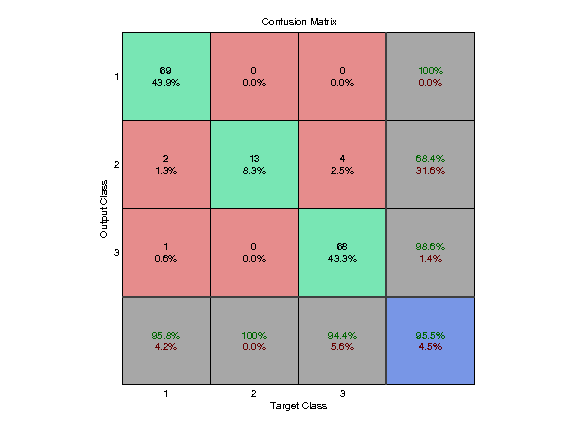
\includegraphics[scale=0.5]{img/mc.png}
				\end{figure}
			\end{frame}
			
			\begin{frame}
				\frametitle{\normalsize Medidas de rendimiento}
				
				\begin{block}{Ratio Correctamente Clasificado (CCR)}
					\begin{itemize}\justifying
						\item \small Cuando hay más de dos clases en el modelo.
						\item \small Se obtiene a partir de la matriz de confusión.
						\item \small Es la suma del número de predicciones correctas dividido por el número total de elementos de la matriz.
					\end{itemize}
					
					\begin{equation}
						\centering
						CCR = \frac{\text{nº de bien clasificados}}{\text{nº total de patrones}} \nonumber
					\end{equation}
				\end{block}
			\end{frame}
				
			\begin{frame}
				\frametitle{\normalsize Medidas de rendimiento}
				
				\begin{block}{Error Absoluto Medio (MAE)}
					\begin{itemize}\justifying
						\item Es una cantidad usada para medir como de buenos son los pronósticos o predicciones de los resultados. Es necesario asignar etiquetas consecutivas a cada una de las $J$ clases de la clasificación ordinal.
					\end{itemize}
					
					\begin{equation}
						\centering
						MAE = \frac{1}{J} \sum_{i=1}^J{\left |{f_i-y_i}\right |} = \sum_{i=1}^J{\left |{e_i}\right |} \nonumber
					\end{equation}
					
					\begin{itemize}\justifying
						\item El error absoluto medio es una media de los errores absolutos, $ e_i = f_i-y_i $, donde $ f_i $ es la predicción e $ y_i $ es el valor verdadero.
					\end{itemize}
				\end{block}
			\end{frame}

	% Analisis del sistema
	\section{Análisis del Sistema}
	
		\subsection{Algoritmo de Regresión Ordinal ORNNet}
		
			\begin{frame}\justifying
				\frametitle{\normalsize Algoritmo de Regresión Ordinal ORNNet}

				La idea de este algoritmo es proyectar los patrones a una línea recta y clasificar según los distintos umbrales de la última capa.\\

				\begin{block}{Modelo de red}
					\begin{itemize}\justifying
						\item El modelo de red neuronal artificial ordinal se basa en:
						\begin{itemize}\justifying
							\item Una capa de entrada.
							\item Dos capas ocultas.
							\item Una capa de salida.
						\end{itemize}
					\end{itemize}
				\end{block}
			\end{frame}
				
			\begin{frame}
				\frametitle{\normalsize Algoritmo de Regresión Ordinal ORNNet}
				
				\begin{figure}[h]
					\centering
					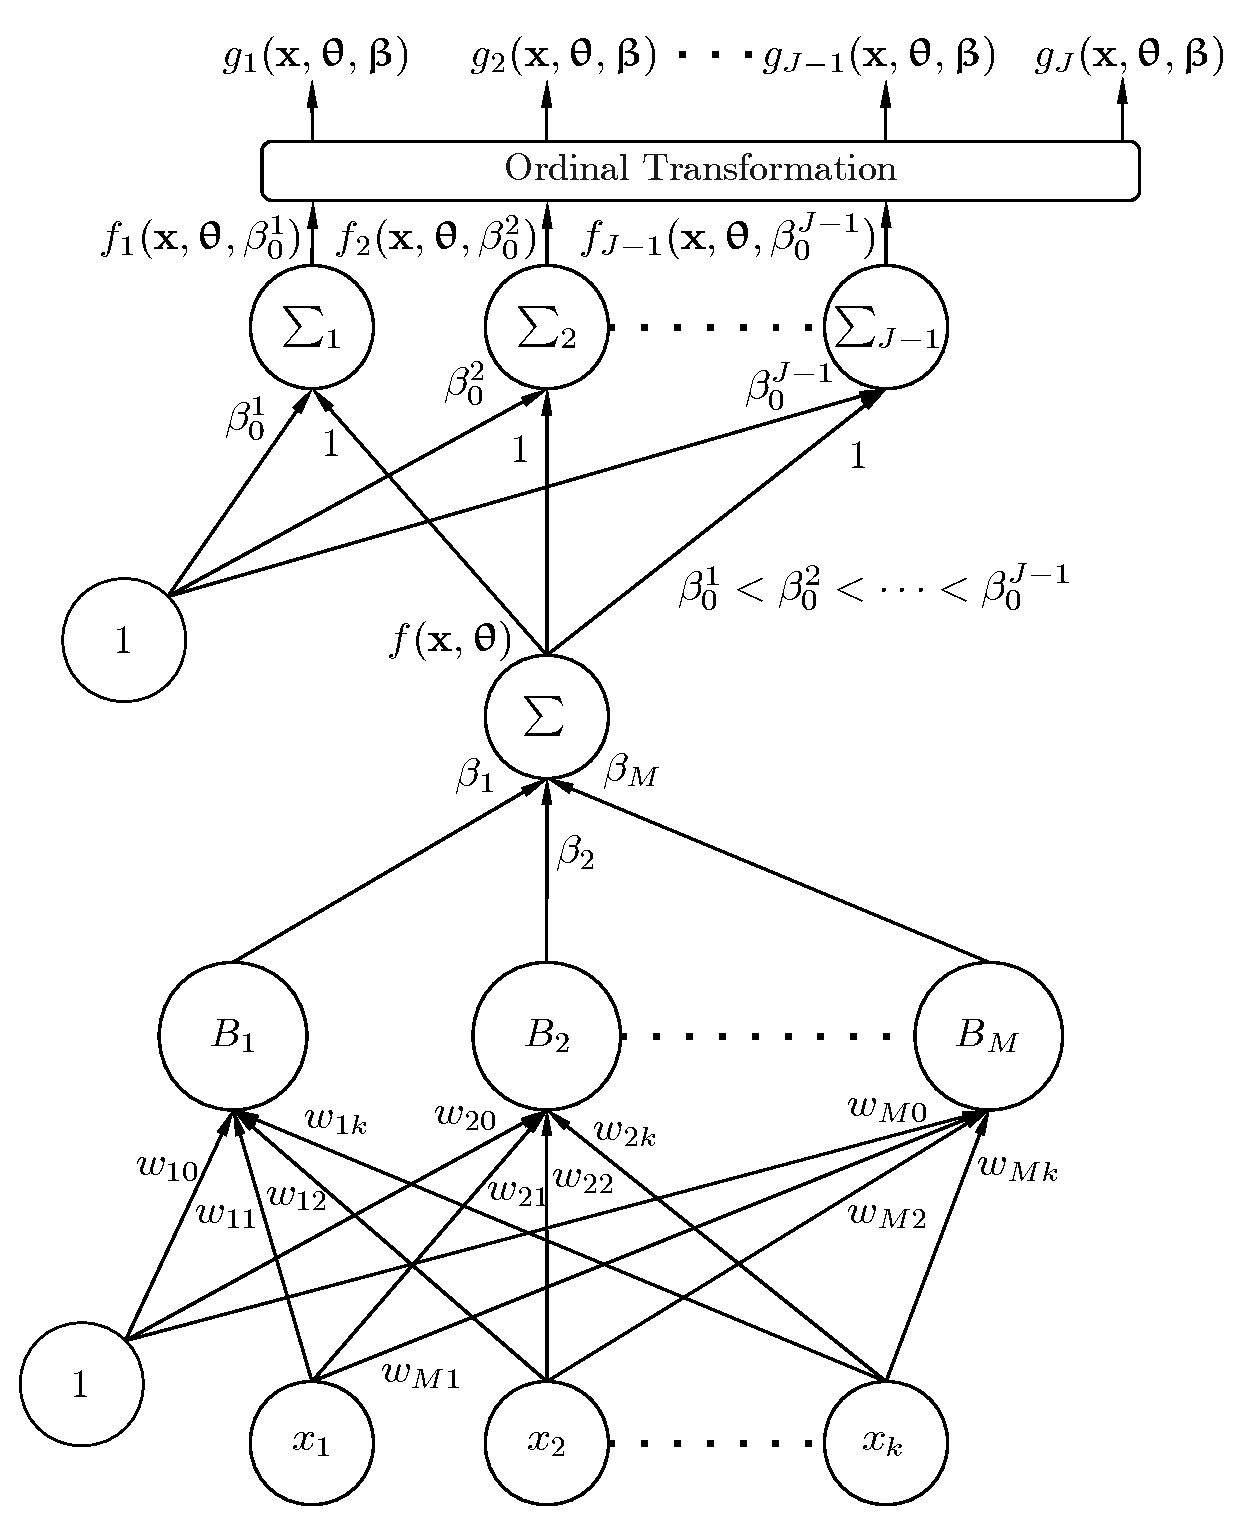
\includegraphics[scale=0.3]{img/ORNNet.pdf}
				\end{figure}
			\end{frame}
				
			\begin{frame}
				\frametitle{\normalsize Algoritmo de Regresión Ordinal ORNNet}
				
				\begin{block}{Capa de entrada}
					\begin{itemize}\justifying
						\item La capa de entrada tomará los valores de las variables de entrenamiento de entrada ($x_1, x_2, ..., x_n$) que al pasar a la siguiente capa generarán nuevos valores ($B_1, B_2, ..., B_M$) haciendo uso de funciones de base sigmoides, utilizando los valores de los pesos ($w_1, w_2, ..., w_i$) en las $M$ funciones de base.
						\item Para obtener los valores de la primera capa oculta se utilizará una función de transferencia (sigmoide), por ejemplo, una \textit{logsig} o \textit{tansig}.
					\end{itemize}
				\end{block}
			\end{frame}
			
			\begin{frame}
				\frametitle{\normalsize Algoritmo de Regresión Ordinal ORNNet}
				
				\begin{figure}[h]
					\centering
					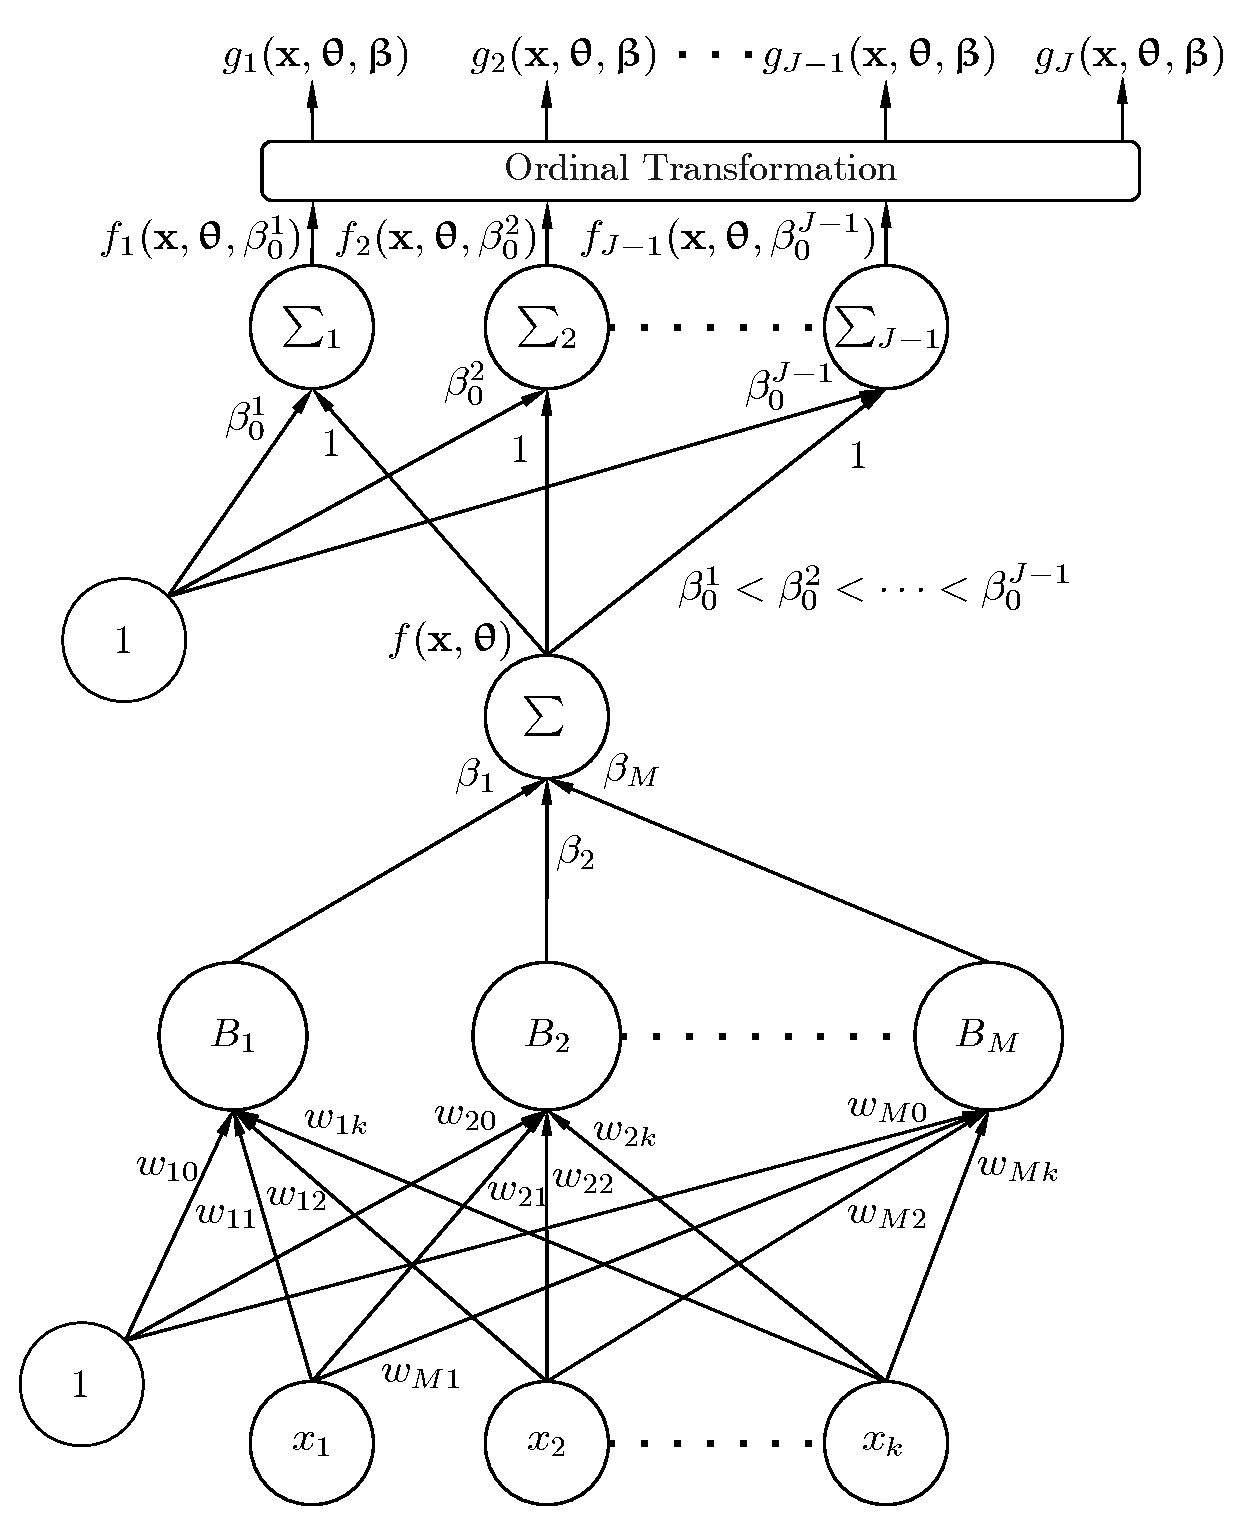
\includegraphics[scale=0.3]{img/ORNNet.pdf}
				\end{figure}
			\end{frame}
				
			\begin{frame}
				\frametitle{\normalsize Algoritmo de Regresión Ordinal ORNNet}
				
				\begin{block}{Capas ocultas}
					\begin{itemize}\justifying
						\item La primera capa oculta obtendrá los nuevos valores de las funciones base a partir de los datos de entrada.
						\item La segunda capa oculta, tendrá solo una neurona asociada a una combinación lineal sin sesgo de las funciones de base.
						\item Esta última capa utilizará la función \textit{purelin} como función de transferencia fija.
					\end{itemize}
				\end{block}
			\end{frame}
			
			\begin{frame}
				\frametitle{\normalsize Algoritmo de Regresión Ordinal ORNNet}
				
				\begin{figure}[h]
					\centering
					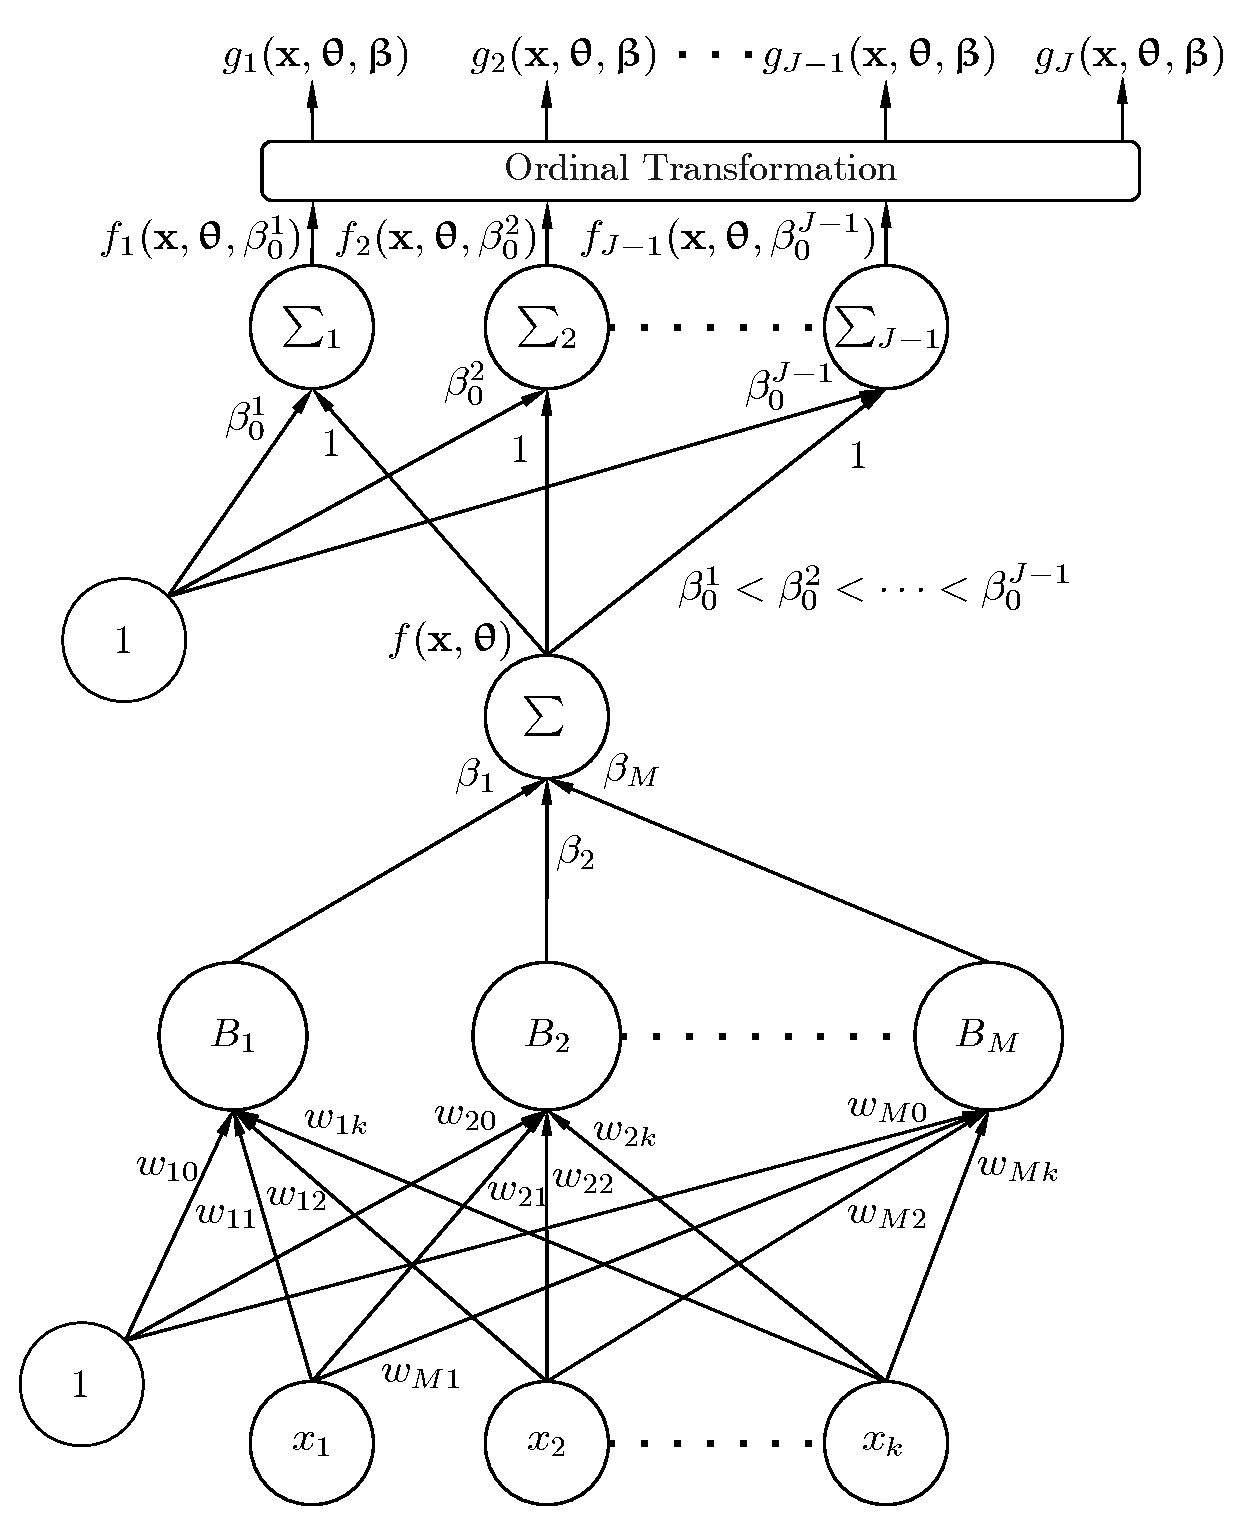
\includegraphics[scale=0.3]{img/ORNNet.pdf}
				\end{figure}
			\end{frame}
				
			\begin{frame}
				\frametitle{\normalsize Algoritmo de Regresión Ordinal ORNNet}
				
				\begin{block}{Capa de salida}
					\begin{itemize}\justifying
						\item Tendrá el mismo número de neuronas que número de clases menos una.
						\item El valor de los pesos se encuentra fijo a 1.
						\item Utilizará la función de transferencia \textit{logsig}.
						\item Las condición que existe en la capa de salida es que el valor de los \textit{sesgos o umbrales} tiene que mantener el orden, es decir, $\beta^1_0< \beta^2_0< \cdots < \beta^{J-1}_0$.
					\end{itemize}
				\end{block}
			\end{frame}
			
			\begin{frame}
				\frametitle{\normalsize Algoritmo de Regresión Ordinal ORNNet}
				
				\begin{figure}[h]
					\centering
					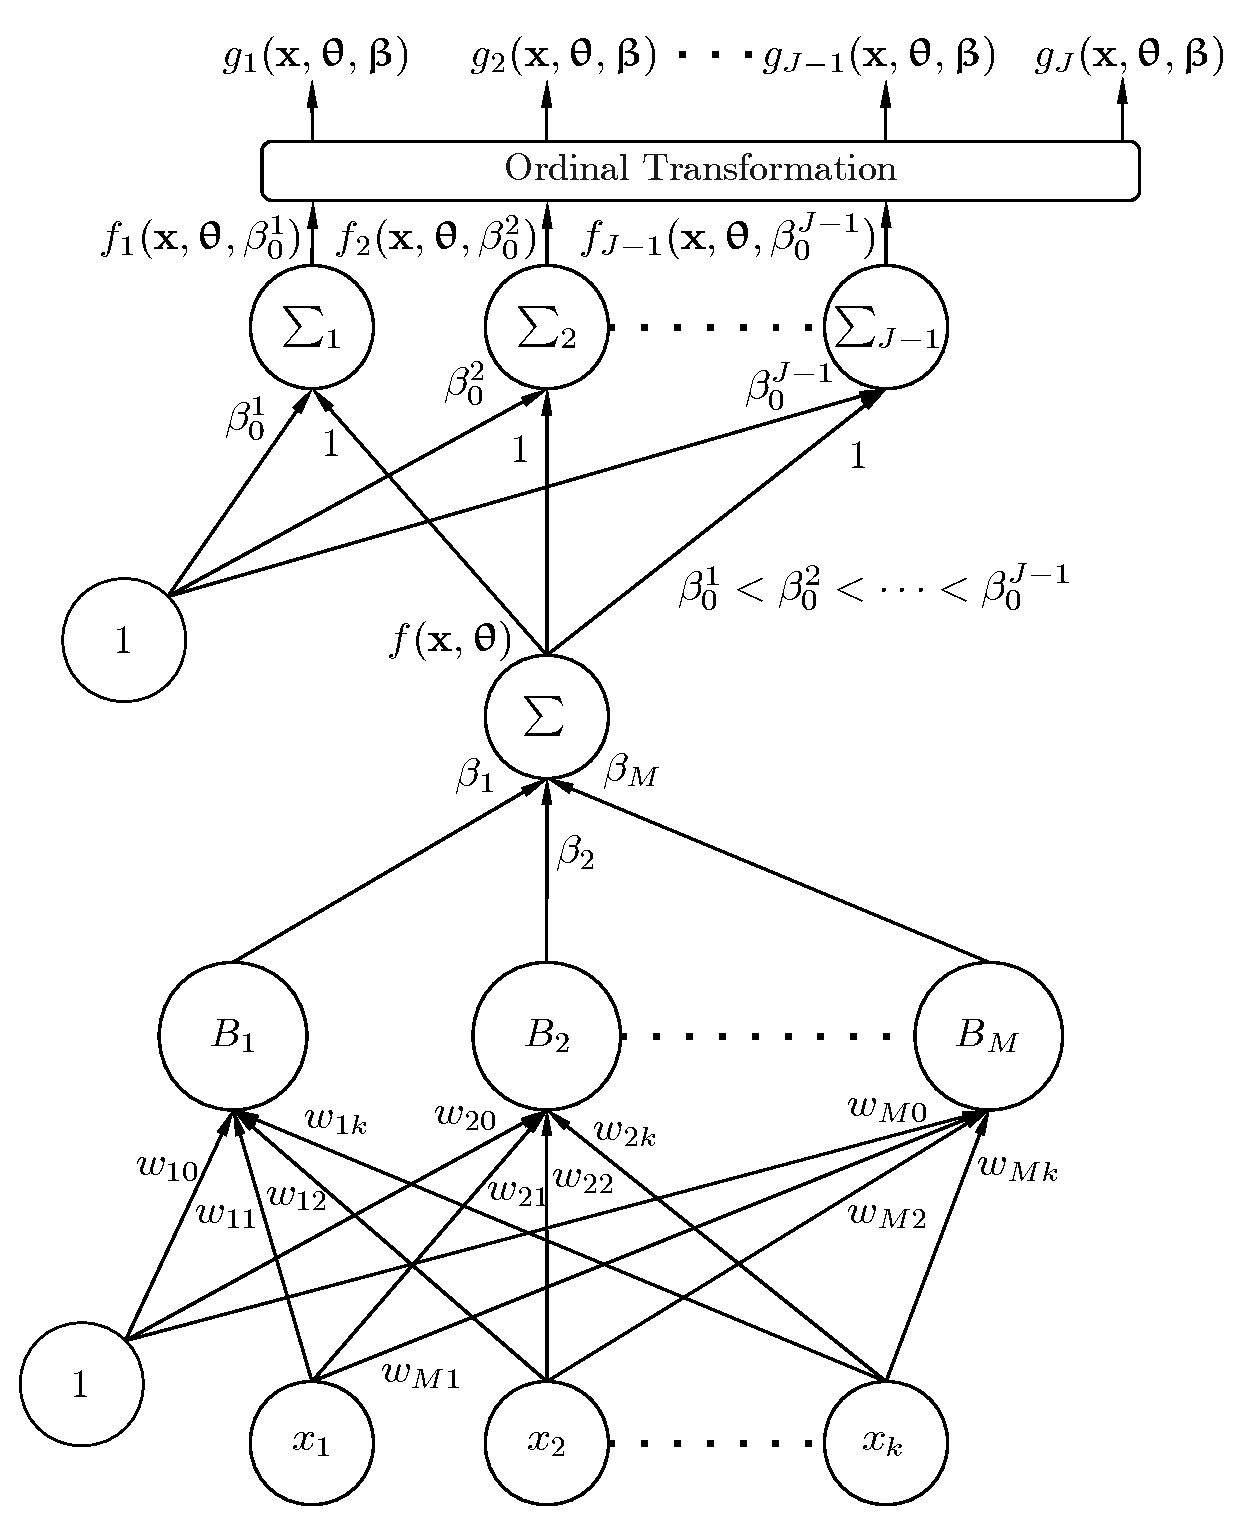
\includegraphics[scale=0.3]{img/ORNNet.pdf}
				\end{figure}
			\end{frame}

		\subsection{Casos de Uso}

			\begin{frame}[allowframebreaks]
				\frametitle{\normalsize Casos de Uso}

				\centering
				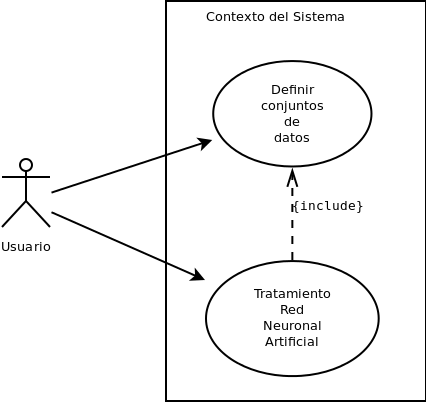
\includegraphics[scale=0.45]{uml/DiagramaContexto.png}
				
				\centering
				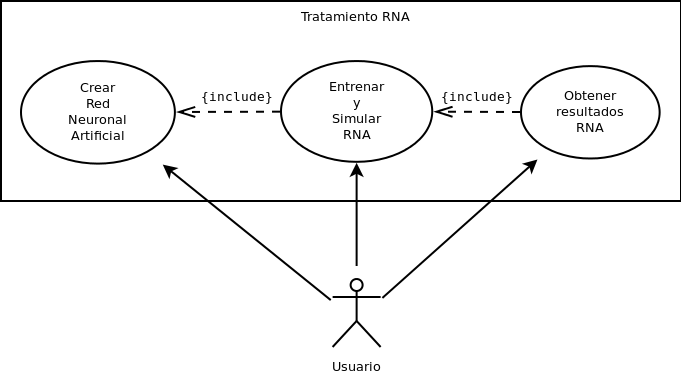
\includegraphics[scale=0.45]{uml/DiagramaNivel1.png}
			\end{frame}

		\subsection{Análisis de la Interfaz}

			\begin{frame}
				\frametitle{\normalsize Análisis de la Interfaz}

				\begin{itemize}\justifying
					\item Estructura atractiva que resulte familiar al usuario.
					\item Manejo fácil e intuitivo.
					\item Acceso a opciones de configuración.
					\item Posibilidad de realizar vuelta atrás para modificar los datos y poder obtener nuevos resultados.
					\item Los resultados obtenidos deben mostrarse de manera lo más parecida posible a como son mostrados en el toolbox \textit{nnet} de Matlab.
				\end{itemize}
			\end{frame}

	\section{Diseño}

		\subsection{Tecnologías}

			\begin{frame}
				\frametitle{\normalsize Tecnologías}
				
				\begin{block}{Matlab}
					\begin{itemize}\justifying
						\item \small Incluye operaciones vectoriales y matriciales que son fundamentales para resolver los problemas científicos y de ingeniería.
						\item \small Ofrece la posibilidad de programar y desarrollar algoritmos más rá-pidamente que con los lenguajes tradicionales porque ya no hay que realizar tareas administrativas de bajo nivel.
						\item \small Es un software multiplataforma y eso facilita que cualquiera pueda tanto hacer desarrollos, como ejecutar programas ya hechos, en su propio sistema operativo.
						\item \small Su toolbox \textit{nnet} (Neural Network Toolbox) proporciona herramientas para el diseño, implementación, visualización y simulación de redes neuronales artificiales.
						\item \small Proporciona la posibilidad de crear Interfaces Gráficas de Usuario
(GUI).
					\end{itemize}
				\end{block}
			\end{frame}

		\subsection{Arquitectura del Sistema}

			\begin{frame}[allowframebreaks]
				\frametitle{\normalsize Arquitectura del Sistema}

				\centering
				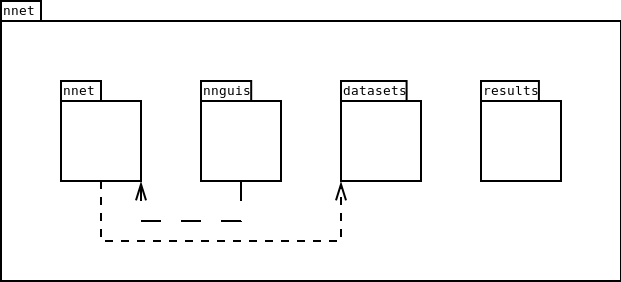
\includegraphics[scale=0.45]{uml/DiagramaPaquetes0.png}
				
				\centering
				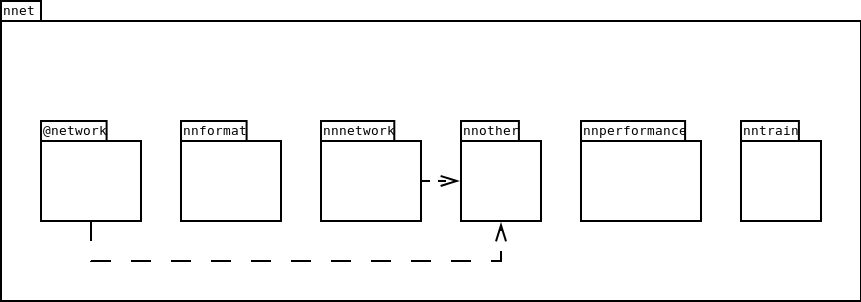
\includegraphics[scale=0.35]{uml/DiagramaPaquetes1.png}
			\end{frame}

	\section{Interfaz Gráfica}

%		\subsection{Pantallas}
%
%			\begin{frame}
%				\frametitle{\normalsize Pantalla Principal}
%				
%				\begin{center}
%					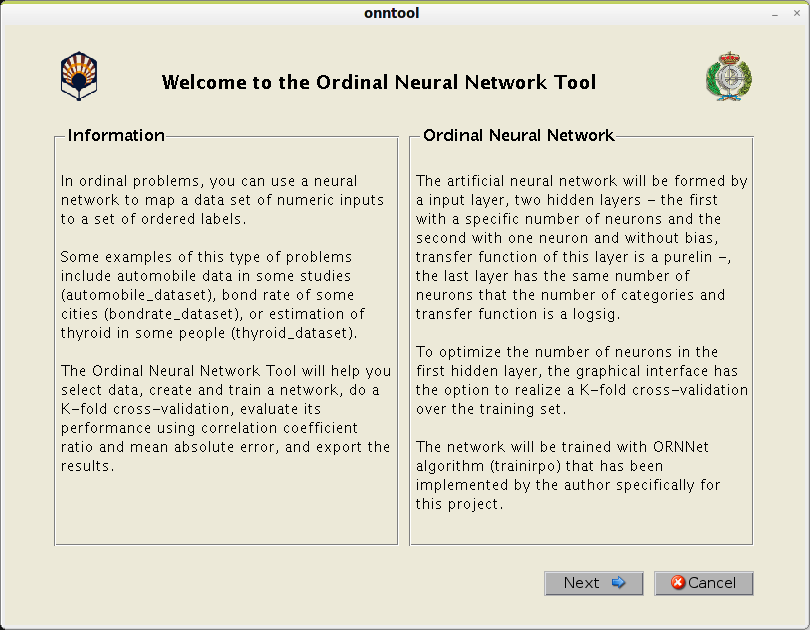
\includegraphics[scale=0.33]{interfaz/interface01.png}
%				\end{center}
%			\end{frame}
%
%			\begin{frame}
%				\frametitle{\normalsize Pantalla de Carga de Datos}
%				
%				\begin{center}
%					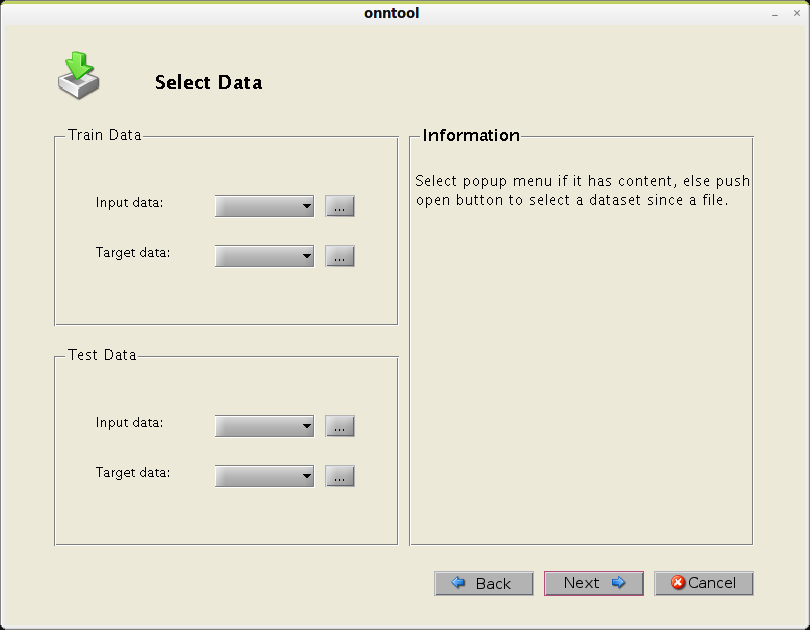
\includegraphics[scale=0.33]{interfaz/interface02.png}
%				\end{center}
%			\end{frame}
%
%			\begin{frame}
%				\frametitle{\normalsize Pantalla de Configuración de la RNA ordinal}
%				
%				\begin{center}
%					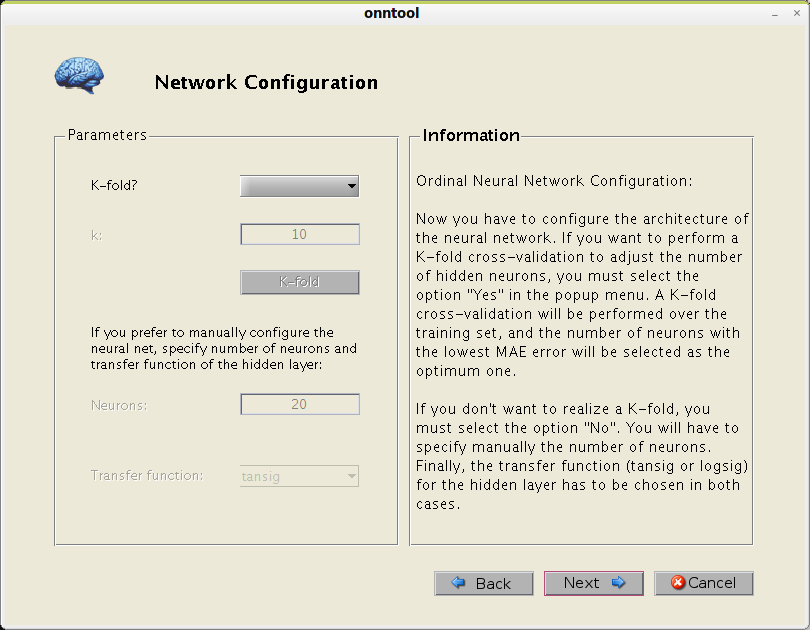
\includegraphics[scale=0.33]{interfaz/interface09.png}
%				\end{center}
%			\end{frame}
%
%			\begin{frame}
%				\frametitle{\normalsize Pantalla de Entrenamiento}
%				
%				\begin{center}
%					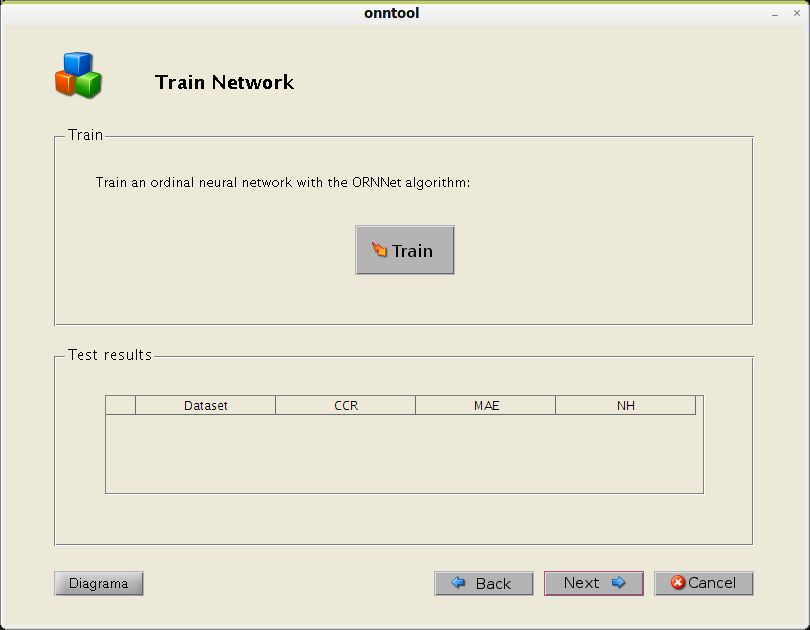
\includegraphics[scale=0.33]{interfaz/interface13.png}
%				\end{center}
%			\end{frame}
%
%			\begin{frame}
%				\frametitle{\normalsize Pantalla de Exportación de Datos}
%				
%				\begin{center}
%					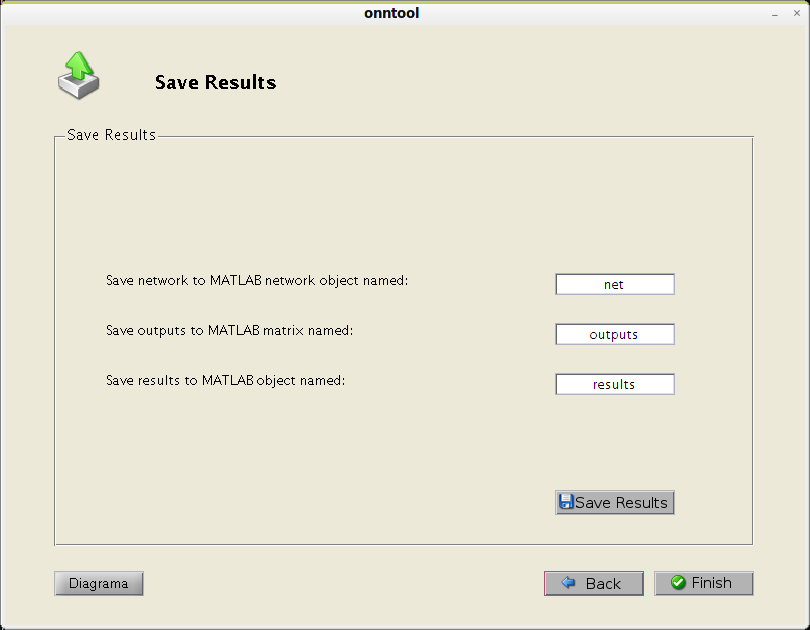
\includegraphics[scale=0.33]{interfaz/interface15.png}
%				\end{center}
%			\end{frame}

		\subsection{Ejemplo de ejecución}

			\begin{frame}
				\frametitle{\normalsize Ejemplo de ejecución}
				
				\begin{center}
					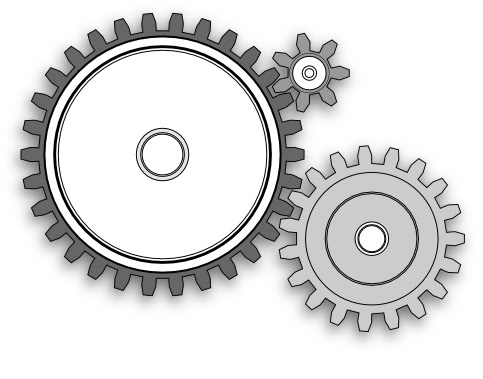
\includegraphics[scale=0.4]{img/ruedadentini.jpg}
				\end{center}
			\end{frame}
	
	\section{Resultados}
	
		\subsection{Resultados de las pruebas}
		
			\begin{frame}\justifying
				\frametitle{\normalsize Resultados de las pruebas}
				
				Los resultados obtenidos por el algoritmo ordinal ORNNet son mejores que los del algoritmo nominal, puesto que:
				
				\begin{itemize}\justifying
					\item En 12 de los conjuntos de datos el \textit{CCR} es mayor que los resultados para el algoritmo nominal.
					\item En 15 conjuntos de datos es menor el valor del \textit{MAE} para el ordinal.
					\item En 11 conjuntos de datos la desviación típica es menor para el \textit{CCR} utilizando la clasificación ordinal frente a la nominal.
					\item Y en 14 ocasiones también es menor la desviación típica para el \textit{MAE} utilizando la clasificación ordinal.
				\end{itemize}
			\end{frame}
	
			\begin{frame}
				\frametitle{\normalsize Resultados de las pruebas}
			
				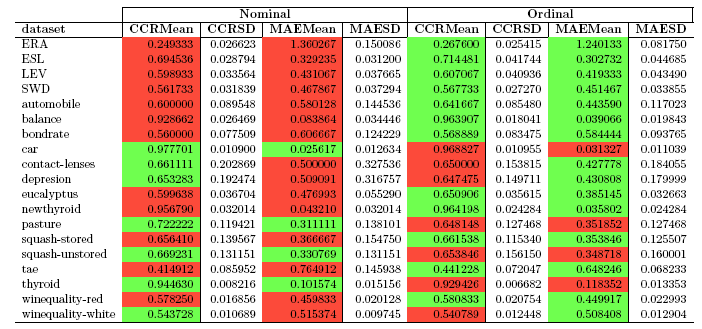
\includegraphics[scale=0.45]{img/resultados.png}
			\end{frame}

	\section{Conclusiones}

		\subsection{Conclusiones del Autor}

			\begin{frame}
				\frametitle{\normalsize Conclusiones de Autor}
				
				\begin{itemize}\justifying
					\item Se ha desarrollado la implementación del algoritmo propuesto de forma teórica (ORNNet) para regresión ordinal basado en redes neuronales artificiales.
					\item Se ha realizado una comparativa de los resultados obtenidos por el clasificador nominal y el ordinal, siendo el ordinal más preciso y estable.
					\item Se ha implementado una interfaz amigable y usable para cualquier tipo de usuario.
					\item Se han modularizado todos los ficheros y funciones para que tenga una compatibilidad e integración completa con el toolbox \textit{nnet} de Matlab.
				\end{itemize}
			\end{frame}

		\subsection{Futuras Mejoras}

			\begin{frame}
				\frametitle{\normalsize Futuras Mejoras}
				
				\begin{itemize}\justifying
					\item Realizar un estudio de los nuevos algoritmos basados en regresión ordinal que aparezcan y, a partir de estos, implementar un nuevo algoritmo que mejorase la efectividad de los resultados obtenidos.
					\item Realizar la adaptación al toolbox \textit{nnet} de Matlab del resto de algoritmos
o desarrollos que el grupo de investigación AYRNA tiene de proyectos o estudios anteriores basados en redes neuronales artificiales.
					\item Mejoras varias en la interfaz:
					\begin{enumerate}\justifying
						\item Añadir la funcionalidad para la realización del método nominal además del ordinal.
						\item Dotar de un aspecto más moderno a los elementos de la interfaz.
						\item Solucionar alguna limitación actual, como mostrar los resultados de cada entrenamiento añadiéndolos en la tabla de resultados.
						\item Soporte para más formatos de archivos de entrada de los conjuntos de datos.
					\end{enumerate}
				\end{itemize}
			\end{frame}

	\section{Bibliografía}
	
		\begin{frame}[allowframebreaks]
			\frametitle{\normalsize Bibliografía}
			
			\begin{thebibliography}{10}
				\bibitem{Ch05}
					W. Chu and S.S. Keerthi.
					\newblock ``New Approaches to Support Vector Ordinal Regression".
					\newblock {\em Proc. 22nd Int. Conf. Machine Learning (ICML ’05)}, pp. 145-152.
					2005.
				
				\bibitem{Lin07}
					L. Lin and H.-T. Lin.
					\newblock ``Ordinal Regression by Extended Binary Classification".
					\newblock {\em Advances in Neural Inform.} Processing Systems, vol. 19, pp. 865-872, MIT Press.
					2007.
	
				\bibitem{Mcc80}
					McCullagh.
					\newblock ``P. Regression models for ordinal data".
					\newblock {\em Journal of the Royal Statistical Society}, Series B (Methodological), 42, 109–142.
					1980.

				\bibitem{Sh03}
					Shashua and A. Levin.
					\newblock ``Ranking with Large Margin Principle: Two Approaches".
					\newblock {\em Advances in Neural Inform.} Processing Systems, vol. 15, 961-968, MIT Press.
					2003.

				\bibitem{RPROP}
					Riedmiller, Martin.
					\newblock ``RPROP - Descriptión and Implmentation Details".
					\newblock {\em University of Karlsruhe.} Technical Report.
					1994.

				\bibitem{iRPROP+}
					Igel, Christian; Hüsken, Michael.
					\newblock ``Empirical evaluation of the improved RPROP learning algorithms".
					\newblock {\em Institut für Neuroinformatik, Ruhr-Universität Bochum.} Germany.
					2001.
			\end{thebibliography}

			\frametitle{\normalsize Bibliografía}
		\end{frame}

\end{document}
